%
% fixpunkte.tex
%
% (c) 2021 Prof Dr Andreas Müller, OST Ostschweizer Fachhochschule
%
\section{Fixpunkte
\label{buch:section:fixpunkte}}
Zu jeder Abbildung $f\colon X\to X$ eines topologischen Raumes in sich
selbst gehört die zugehörige lineare Abbildung $f_*\colon H_*(X)\to H_*(X)$
der Homologiegruppen.
Diese linearen Abbildungen sind im Allgemeinen viel einfacher zu
analysieren als Abbildungen topologischer Räume.
%Zum Beispiel soll in Abschnitt~\ref{buch:subsection:lefshetz}
%die Lefshetz-Spurformel abgeleitet werden, die eine Aussagen darüber
%ermöglicht, ob eine Abbildung einen Fixpunkt haben kann.
%In Abschnitt~\ref{buch:subsection:brower} wird gezeigt wie man damit 
%den Browerschen Fixpunktsatz beweisen kann, der besagt, dass jede
%Abbildung eines Einheitsballs in sich selbst immer einen Fixpunkt hat.

%\subsection{Brower-Fixpunktsatz
%\label{buch:subsection:brower}}
%
%\begin{satz}[Brower]
%\end{satz}

\rhead{Fixpunkte}

%\subsection{Lefshetz-Fixpunktsatz
%\label{buch:subsection:lefshetz}}
Eine Selbstabbildung $f_*\colon C_*\to C_*$ von Kettenkomplexen führt auf
eine Selbstabbildung der Homologiegruppen $H(f)\colon H(C)\to H(C)$.
Da sowohl $H_k$ wie auch $C_k$ endlichdimensionale Vektorräume sind, 
ist die Spur von $H_k(f)$ wohldefiniert.

\begin{definition}
Die {\em Lefshetz-Zahl} einer Abbildung $f$ von Kettenkomplexen ist
\begin{equation}
\lambda(f)
=
\sum_{k=0}^\infty
(-1)^k \operatorname{Spur}f_k
=
\sum_{k=0}^\infty 
(-1)^k \operatorname{Spur}(H_k(f)).
\label{buch:homologie:lefschetz-zahl}
\end{equation}
\end{definition}

Die zweite Darstellung  der Lefshetz-Zahl auf der rechten Seite ist
meistens viel leichter zu berechnen als die erste.
Die einzelnen Vektorräume eines Kettenkomplexes können haben typischerweise
eine hohe Dimension, so hoch wie die Anzahl der Simplizes der Triangulation.
Die Homologiegruppen dagegen haben typischerweise sehr viel kleinere 
Dimension, die Matrizen $H_k(f)$ sind also relativ klein.
Es ist aber nicht klar, dass beide Berechnungsmethoden für die 
Lefshetz-Zahl auf das gleiche Resultat führen müssen.

\begin{figure}
\centering
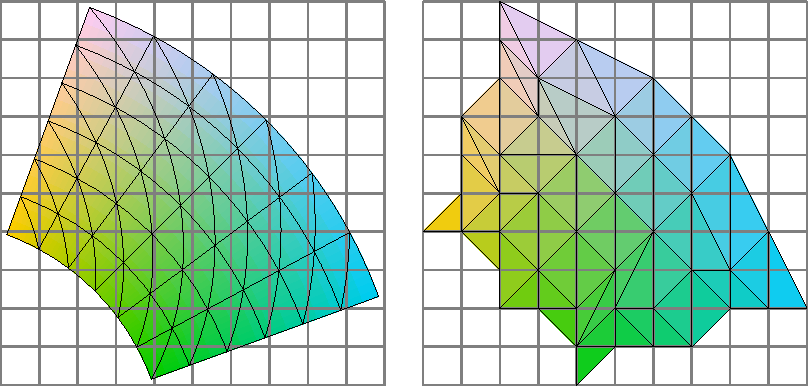
\includegraphics[width=\textwidth]{chapters/95-homologie/images/approximation.pdf}
\caption{Stückweise lineare Approximation einer Abbildung derart,
dass die Bildpunkte von Knoten auf Gitterpunkte fallen.
Die Abbildung wird damit zu einer Abbildung von Polyedern und
die induzierte Abbildung der Kettenkomplexe lässt sich direkt berechnen.
Wenn die Auflösung des Gitters klein genug ist, hat die Approximation
einer Abbildung ohne Fixpunkte immer noch keine Fixpunkte.
\label{buch:homologie:fig:simplapprox}}
\end{figure}%

\begin{proof}[Beweis]
Im Abschnitt~\ref{buch:subsection:induzierte-abbildung} wurde gezeigt,
dass die Basis des Komplexes immer so gewählt werden kann, dass für
die Spuren der Teilmatrizen von $f_k$ die
Formel~\eqref{buch:homologie:eqn:spur} gilt.
Damit kann jetzt die alternierenden Summe der Spuren von $f_k$ ermittelt
werden:
\begin{align*}
\sum_{k=0}^\infty (-1)^k\operatorname{Spur}(f_k)
&=
\sum_{k=0}^\infty (-1)^k\operatorname{Spur}(f_{k,B})
+
\sum_{k=0}^\infty (-1)^k\operatorname{Spur}(f_{k,Z})
+
\sum_{k=0}^\infty (-1)^k\operatorname{Spur}(f_{k-1,B})
\\
&=
\sum_{k=0}^\infty (-1)^k\operatorname{Spur}(f_{k,B})
+
\sum_{k=0}^\infty (-1)^k\operatorname{Spur}(f_{k,Z})
-
\sum_{k=0}^\infty (-1)^k\operatorname{Spur}(f_{k,B})
\\
&=
\sum_{k=0}^\infty (-1)^k\operatorname{Spur}(f_{k,Z}).
\intertext{Die Abbildung $H_k(f)$ hat $f_{k,Z}$ als Matrix, also ist
die letzte Form gleichbedeutend mit}
&=
\sum_{k=0} (-1)^k\operatorname{Spur} H_k(f).
\end{align*}
Damit ist die Formel
\eqref{buch:homologie:lefschetz-zahl}
bewiesen.
\end{proof}

Die Lefshetz-Zahl ist eine Invariante einer topologischen Abbildung,
die Aussagen über Fixpunkte zu machen erlaubt.

\begin{satz}
Ist $f\colon X\to X$ eine Selbstabbildung eines kompakten Polyeders und
ist $\lambda(f) \ne 0$, dann hat $f$ einen Fixpunkt.
\end{satz}

Im Folgenden soll nur ein heuristisches Argument gegeben werden, warum
ein solcher Satz wahr sein könnte.


Wenn eine Abbildung keinen Fixpunkt hat, dann ist $f(x) \ne x$ für alle
Punkte von $X$.
Da $X$ kompakt ist, gibt es einen minimalen Abstand $d$ zwischen $f(x)$ und $x$.
Wenn man also für $X$ eine Triangulation wählt, die wesentlich feiner ist
als dieser minimale Abstand, dann wird kein Simplex der Triangulation auf
Punkte im selben Simplex oder in einem Nachbarsimplex abgebildet wird.
Indem man nötigenfalls die Triangulation nochmals verfeinert, kann man auch
genügend Platz schaffen, dass man die Abbildung $f$ etwas modifizieren kann,
so dass auch die deformierte Abbildung immer noch diese Eigenschaft hat.
Die Abbildung~\ref{buch:homologie:fig:simplapprox} illustriert, wie eine
Abbildung durch eine andere approximiert werden kann, die die Triangulation
im Bildraum respektiert.

Die zugehörige Abbildung des Kettenkomplexes der Triangulation hat damit
die Eigenschaft, dass kein Basisvektor auf sich selbst abgebildet wird.
Die Matrix der Abbildung hat daher keine Nullen auf der Diagonalen, und
damit ist auch die Spur dieser Abbildung Null: $\operatorname{Spur}(H_k(f))=0$
für alle $k$.
Erst recht ist die Lefshetz-Zahl $\lambda(f)=0$.
Wenn also die Lefshetz-Zahl verschieden ist von Null, dann muss $f$
notwendigerweise einen Fixpunkt haben.

Dieser Fixpunktsatz zeigt, dass die Topologie eines Raumes $X$ Situationen
erzwingen kann, wo eine Abbildung $f\colon X\to X$ einen Fixpunkt, oder
anders ausgedrückt ein Lösung der Gleichung $f(x)=x$ haben muss.
Diese Eigenschaft bleibt sogar bei Deformation erhalten.


